\documentclass[aspectratio=169]{beamer}
\usepackage{fontspec}

% Tipografías de la Identidad Visual
\setmainfont{Inter}
\setsansfont{Inter}
\setmonofont{JetBrains Mono}
\newfontfamily\titlefont{Montserrat}[BoldFont={Montserrat Bold}]

% Colores de la Identidad Visual
\definecolor{AzulMarino}{HTML}{1A365D}
\definecolor{GrisPizarra}{HTML}{4A5568}
\definecolor{BlancoNieve}{HTML}{F7FAFC}
\definecolor{VerdeAzulado}{HTML}{319795}

% Aplicación de colores a Beamer
\setbeamercolor{palette primary}{bg=AzulMarino, fg=BlancoNieve}
\setbeamercolor{palette secondary}{bg=VerdeAzulado, fg=BlancoNieve}
\setbeamercolor{palette tertiary}{bg=GrisPizarra, fg=BlancoNieve}
\setbeamercolor{structure}{fg=AzulMarino}
\setbeamercolor{background canvas}{bg=BlancoNieve}
\setbeamercolor{normal text}{fg=GrisPizarra}

\setbeamerfont{title}{family=\titlefont, series=\bfseries, size=\Huge}
\setbeamerfont{frametitle}{family=\titlefont, series=\bfseries, size=\LARGE}

\usepackage[utf8]{inputenc}
\usepackage{graphicx}
\usepackage{amsmath}

\title{Modelos de Regresión y Regularización}
\subtitle{Predicción Continua (Teoría)}
\author{Clase Teórica - Semana 4}
\date{}

\begin{document}

\begin{frame}
    \titlepage
\end{frame}

\begin{frame}{El Cordel Elástico (Regresión Lineal)}
    Imagina tachuelas en una madera. Intentamos colocar un cordel elástico estirado (una línea recta) de forma que pase lo más cerca posible de todas las tachuelas.
    
    \begin{itemize}
        \item \textbf{Mínimos Cuadrados (OLS):} El algoritmo minimiza la distancia al cuadrado entre el cordel (predicción) y la tachuela (realidad).
        \item \textbf{\textcolor{AzulMarino}{Problema:}} Si los datos forman una montaña rusa, un cordel rígido fallará miserablemente (Underfitting).
    \end{itemize}
\end{frame}

\begin{frame}{La Montaña Rusa (Polynomial Features)}
    Para solucionar el \textit{Underfitting}, le damos al cordel la habilidad matemática de doblarse:
    
    $$y = w_0 + w_1 x + w_2 x^2 + w_3 x^3$$
    
    \begin{alertblock}{¡Cuidado con el Overfitting!}
    Si le damos demasiada flexibilidad (ej. grado 100), el cordel se volverá loco tratando de tocar cada tachuela a la perfección, pero fallará al predecir datos futuros.
    \end{alertblock}
\end{frame}

\begin{frame}{Multicolinealidad y el VIF}
    Si le damos a la máquina el \textit{Alto de la pantalla} y el \textit{Ancho de la pantalla} al mismo tiempo, como ambos crecen proporcionalmente (16:9), la matemática de OLS se rompe por información duplicada.
    \vspace{0.3cm}
    
    \textbf{Factor de Inflación de Varianza (VIF):} Mide qué tan redundante es una variable. Si VIF $> 10$, ¡tenemos problemas!
\end{frame}

\begin{frame}{La Mochila de Campamento (Regularización)}
    \begin{columns}
        \column{0.5\textwidth}
        \textbf{\textcolor{AzulMarino}{Inspector Lasso (L1)}} \\
        Severo. Si llevas objetos redundantes en la mochila, te obliga a botarlos a la basura (fuerza los coeficientes exactamente a \textbf{cero}). \\
        \textit{Ideal para selección de características.}
        
        \column{0.5\textwidth}
        \textbf{\textcolor{VerdeAzulado}{Inspector Ridge (L2)}} \\
        Precavido. No tira nada, pero te obliga a hacer todos los objetos miniatura (encoge los coeficientes sin llegar a cero). \\
        \textit{Ideal para multicolinealidad.}
    \end{columns}
\end{frame}

\begin{frame}{El Path de Coeficientes de Lasso}
    \begin{center}
        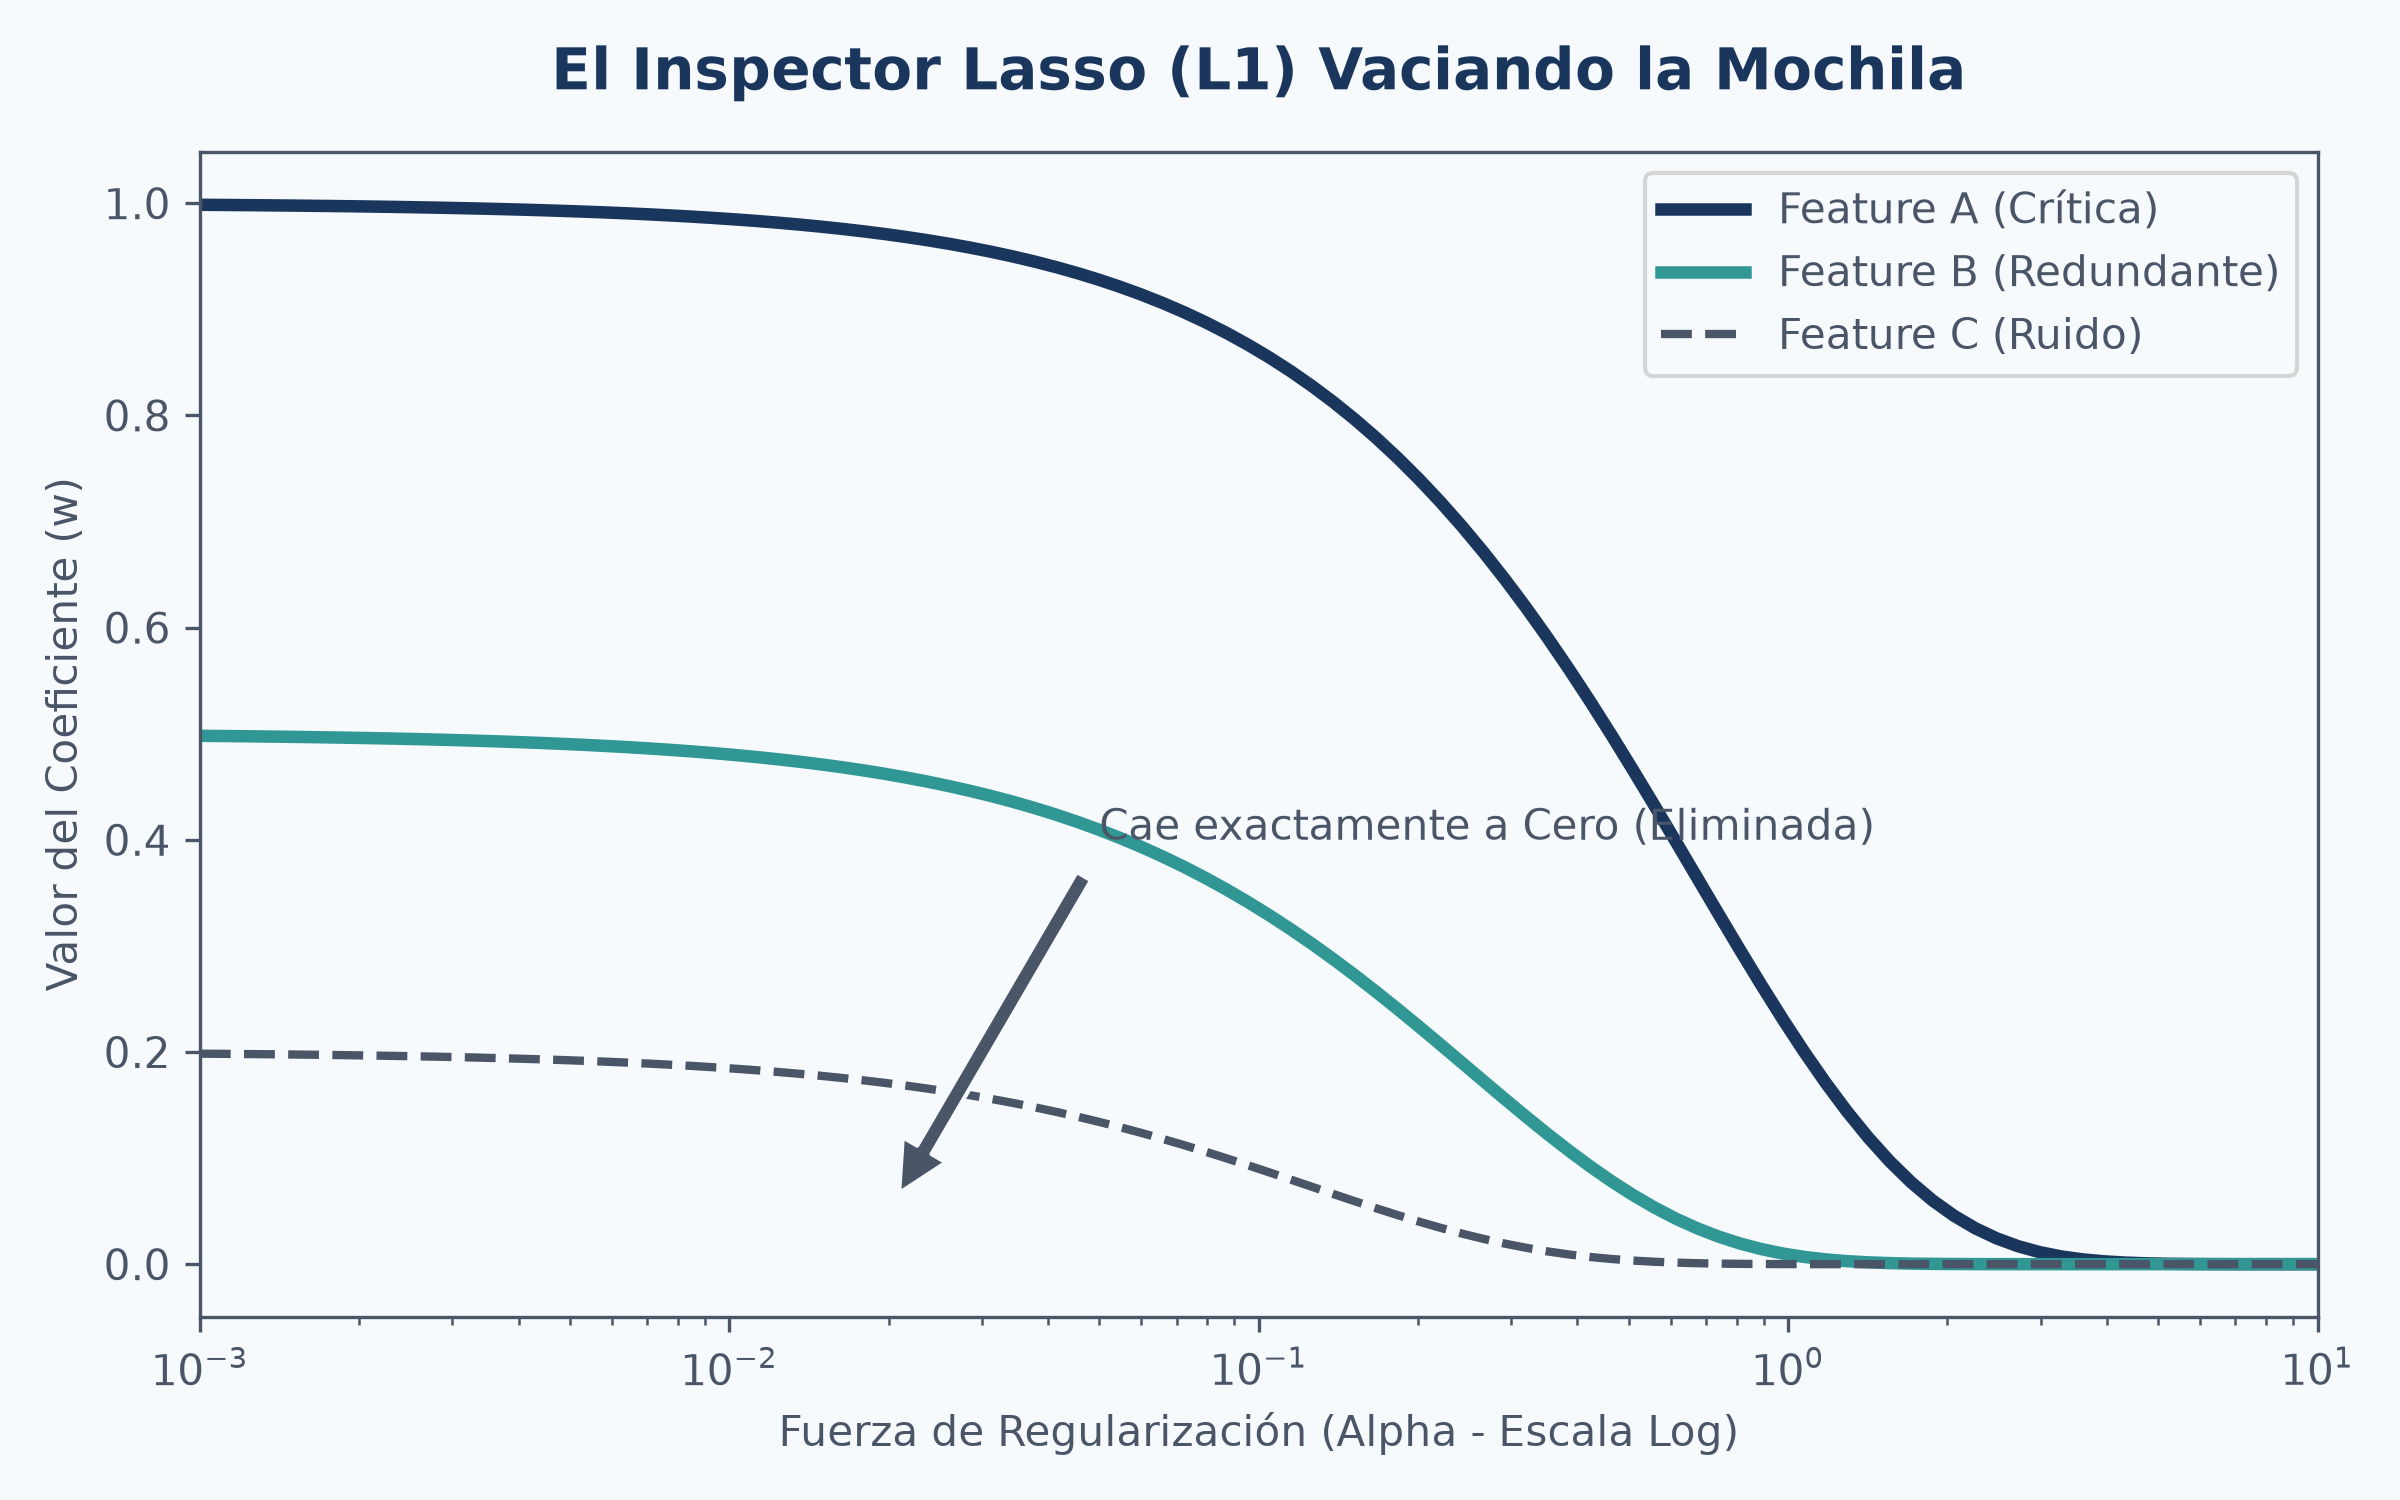
\includegraphics[width=0.6\textwidth]{lasso_path.png}
    \end{center}
    A medida que la penalización (Alpha) sube, Lasso elimina las variables inútiles.
\end{frame}

\end{document}
